\pdfminorversion=4 % for acroread
%\documentclass[aspectratio=169,t,xcolor={usenames,dvipsnames}]{beamer}
\documentclass[aspectratio=169,t,handout,xcolor={usenames,dvipsnames}]{beamer}
\usepackage{../beamerstyle}
\usepackage{dsfont}
\usepackage{bm}
\usepackage[english]{babel}
\usepackage[utf8]{inputenc}
\usepackage{graphicx}
\usepackage{algorithm}
\usepackage[ruled,vlined,algo2e,linesnumbered]{algorithm2e}
%\usepackage[boxed,vlined]{algorithm2e}
\usepackage{hyperref}
\usepackage{booktabs}
\usepackage{mathtools}

\usepackage{amsmath,amssymb}
\usepackage{listings}
\lstset{frame=lines,framesep=3pt,numbers=left,numberblanklines=false,basicstyle=\ttfamily\small}

\usepackage{subfig}
\usepackage{multicol}
%\usepackage{appendixnumberbeamer}
%
\usepackage{tcolorbox}

\usepackage{pgfplots}
\usepackage{tikz}
\usetikzlibrary{trees} 
\usetikzlibrary{shapes.geometric}
\usetikzlibrary{positioning,shapes,shadows,arrows,calc,mindmap}
\usetikzlibrary{positioning,fadings,through}
\usetikzlibrary{decorations.pathreplacing}
\usetikzlibrary{intersections}
\usetikzlibrary{positioning,fit,calc,shadows,backgrounds}
\pgfdeclarelayer{background}
\pgfdeclarelayer{foreground}
\pgfsetlayers{background,main,foreground}
\tikzstyle{activity}=[rectangle, draw=black, rounded corners, text centered, text width=8em]
\tikzstyle{data}=[rectangle, draw=black, text centered, text width=8em]
\tikzstyle{myarrow}=[->, thick, draw=black]

% Define the layers to draw the diagram
\pgfdeclarelayer{background}
\pgfdeclarelayer{foreground}
\pgfsetlayers{background,main,foreground}

%\usepackage{listings}
%\lstset{numbers=left,
%  showstringspaces=false,
%  frame={tb},
%  captionpos=b,
%  lineskip=0pt,
%  basicstyle=\ttfamily,
%%  extendedchars=true,
%  stepnumber=1,
%  numberstyle=\small,
%  xleftmargin=1em,
%  breaklines
%}

 
\definecolor{blue}{RGB}{0, 74, 153}

\usetheme{Boadilla}
%\useinnertheme{rectangles}
\usecolortheme{whale}
\setbeamercolor{alerted text}{fg=blue}
\useoutertheme{infolines}
\setbeamertemplate{navigation symbols}{\vspace{-5pt}} % to lower the logo
\setbeamercolor{date in head/foot}{bg=white} % blue
\setbeamercolor{date in head/foot}{fg=white}
\setbeamercolor{author  in head/foot}{bg=white} %blue
\setbeamercolor{title in head/foot}{bg=white} % blue
\setbeamercolor{title}{fg=white, bg=blue}
\setbeamercolor{block title}{fg=white,bg=blue}
\setbeamercolor{block body}{bg=blue!10}
\setbeamercolor{frametitle}{fg=white, bg=blue}
\setbeamercovered{invisible}

\makeatletter
\setbeamertemplate{footline}
{
  \leavevmode%
  \hbox{%
  \begin{beamercolorbox}[wd=.333333\paperwidth,ht=2.25ex,dp=1ex,center]{author in head/foot}%
%    \usebeamerfont{author in head/foot}\insertshortauthor
  \end{beamercolorbox}%
  \begin{beamercolorbox}[wd=.333333\paperwidth,ht=2.25ex,dp=1ex,center]{title in head/foot}%
    \usebeamerfont{title in head/foot}\insertshorttitle
  \end{beamercolorbox}%
  \begin{beamercolorbox}[wd=.333333\paperwidth,ht=2.25ex,dp=1ex,right]{date in head/foot}%
    \usebeamerfont{date in head/foot}\insertshortdate{}\hspace*{2em}
%    \insertframenumber\hspace*{2ex} 
  \end{beamercolorbox}}%
  \vskip0pt%
}
\makeatother

%\pgfdeclareimage[height=1.2cm]{automl}{images/logos/automl.png}
%\pgfdeclareimage[height=1.2cm]{freiburg}{images/logos/freiburg}

%\logo{\pgfuseimage{freiburg}}

\renewcommand{\comment}[1]{
	\noindent
	%\vspace{0.25cm}
	{\color{red}{\textbf{TODO:} #1}}
	%\vspace{0.25cm}
}
\newcommand{\notefh}[1]{\textcolor{red}{\textbf{FH:} #1}}
\renewcommand{\comment}[1]{}
\newcommand{\hide}[1]{}
\newcommand{\cemph}[2]{\emph{\textcolor{#1}{#2}}}

\newcommand{\lit}[1]{{\footnotesize\color{black!60}[#1]}}

\newcommand{\litw}[1]{{\footnotesize\color{blue!20}[#1]}}


\newcommand{\myframe}[2]{\begin{frame}[c]{#1}#2\end{frame}}
\newcommand{\myframetop}[2]{\begin{frame}{#1}#2\end{frame}}
\newcommand{\myit}[1]{\begin{itemize}#1\end{itemize}}
\newcommand{\myblock}[2]{\begin{block}{#1}#2\end{block}}


\newcommand{\votepurple}[1]{\textcolor{Purple}{$\bigstar$}}
\newcommand{\voteyellow}[1]{\textcolor{Goldenrod}{$\bigstar$}}
\newcommand{\voteblue}[1]{\textcolor{RoyalBlue}{$\bigstar$}}
\newcommand{\votepink}[1]{\textcolor{Pink}{$\bigstar$}}

\newcommand{\diff}{\mathop{}\!\mathrm{d}}
\newcommand{\refstyle}[1]{{\small{\textcolor{gray}{#1}}}}
\newcommand{\hands}[0]{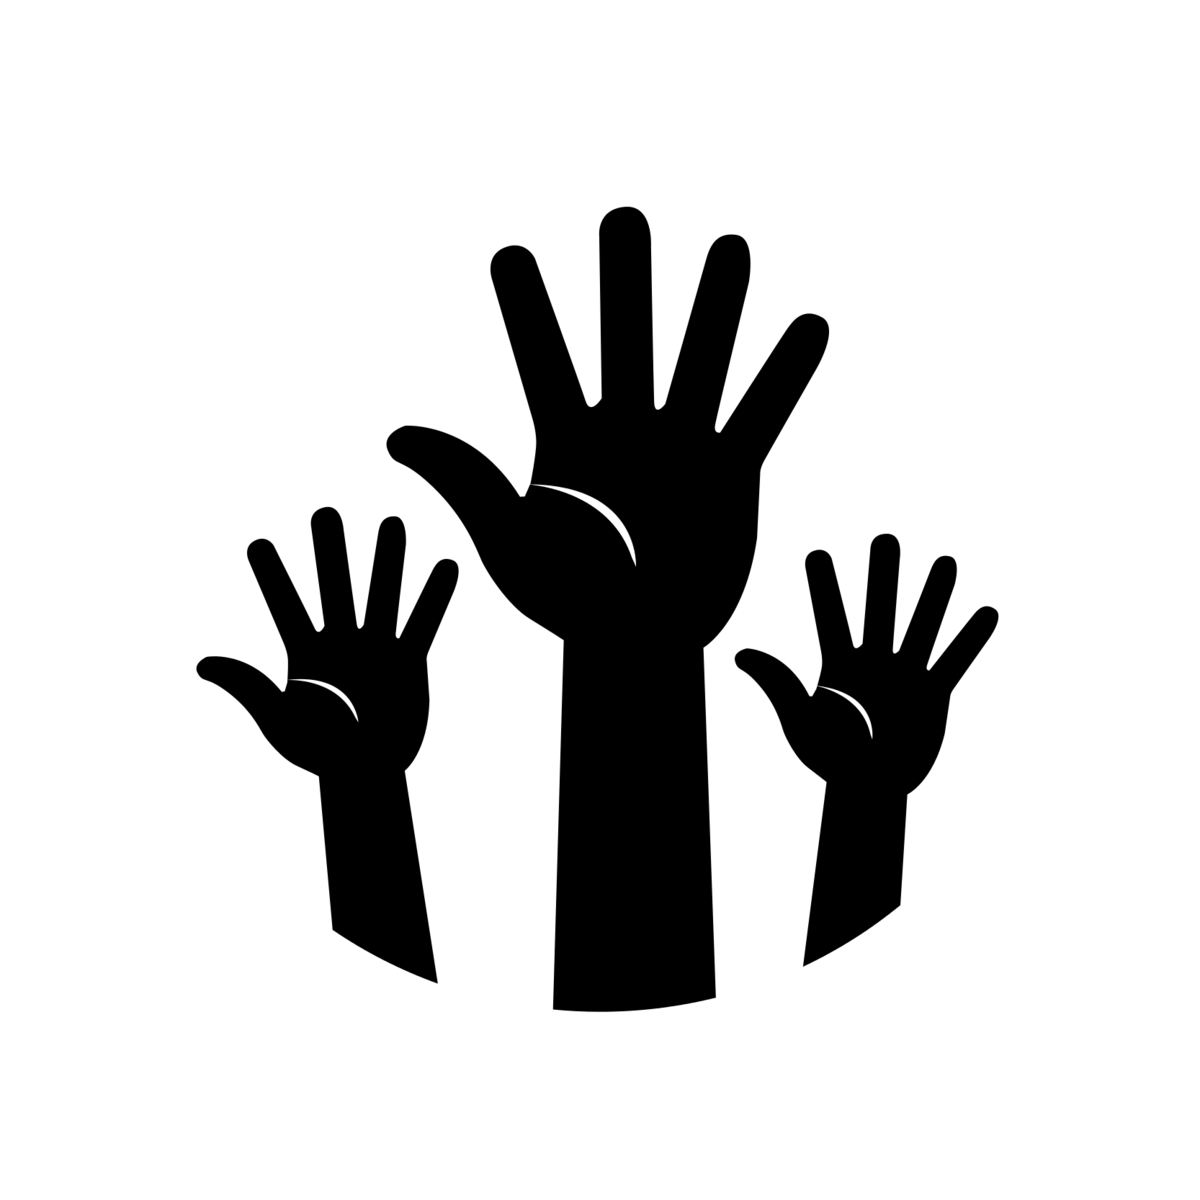
\includegraphics[height=1.5em]{images/hands}}
\newcommand{\transpose}[0]{{\textrm{\tiny{\sf{T}}}}}
\newcommand{\norm}{{\mathcal{N}}}
\newcommand{\cutoff}[0]{\kappa}
\newcommand{\instD}[0]{\dataset}
\newcommand{\insts}[0]{\mathcal{I}}
\newcommand{\inst}[0]{i}
\newcommand{\instI}[1]{i^{(#1)}}

% Iteration specific instance of variable/function/anything
% Introduced in the BO section, but moved up here to make it available within other macros
\newcommand{\iter}[2][\bocount]{{#2}^{(#1)}}

%--------HPO parameter macros-----------

% Parameter Configuration Space
\newcommand{\pcs}[0]{\pmb{\Lambda}}

% ???
\newcommand{\bx}[0]{\conf}

% Parameter Configuration
\newcommand{\conf}[0]{\pmb{\lambda}}

% Final Configuration
\newcommand{\finconf}[0]{\pmb{\hat{\lambda}}}

% Configuration corresponding to a given iteration -- better use \iter!
\newcommand{\confI}[1]{{\conf}^{(#1)}}

% Default Configuration
\newcommand{\defconf}[0]{{\conf}_{\text{def}}}

% Incumbent Configuration
\newcommand{\incumbent}[1][\bocount]{\iter[#1]{\finconf}}

% Optimal Configuration
\newcommand{\optconf}[0]{{\conf}^*}

% Configuration Space
\newcommand{\confs}[0]{\pcs}

%----------------------------------------

%\newcommand{\vlambda}[0]{\bm{\lambda}}
%\newcommand{\vLambda}[0]{\bm{\Lambda}}
\newcommand{\dataset}[0]{\mathcal{D}}
\newcommand{\datasets}[0]{\mathbf{D}}
\newcommand{\loss}[0]{L}
\newcommand{\risk}{\mathcal{R}}
\newcommand{\riske}{\mathcal{R}_{\text{emp}}}
\newcommand{\cost}[0]{c}
\newcommand{\costI}[1]{c^{(#1)}}

% Gaussian Process
\newcommand{\gp}{\mathcal{G}}
% Family of Objective Functions
\newcommand{\objF}{F}

%---------------BO Macros------------------

% BO loop counter
\newcommand{\bocount}{t}
% BO loop counter max, the counter runs from 1 to this value
\newcommand{\bobudget}{T}
% BO loop observation
\newcommand{\obs}[1][\conf]{\cost({#1})}
% BO loop observation space
\newcommand{\obsspace}{\mathcal{Y}}
% BO loop next observation
\newcommand{\bonextobs}{\obs[\iter{\conf}]}
% Acquisition Function, no args
\newcommand{\acq}{u}
% Standard Normal PDF
\newcommand{\pdf}{\phi}
% Standard Normal CDF
\newcommand{\cdf}{\Phi}
% Mean
\newcommand{\mean}{\mu}
% Standard Deviation
\newcommand{\stddev}{\sigma}
% Variance
\newcommand{\variance}{\sigma^2}
% Noise
\newcommand{\noise}{\nu}
% BO loop next selected sample
\newcommand{\bonextsample}{\confI{\bocount}}

% Single hyperparameter
\newcommand{\hyperparam}{\lambda}

% Single hyperparameter within a hyperparameter configuration
\newcommand{\hyperparami}[1][i]{{\hyperparam}_#1}

% Full definition of final configuration
\newcommand{\finconffull}{\incumbent[\bobudget]}

% Dataset
\newcommand{\datasetHPO}{{\dataset}_{HPO}}

% Dataset definition
\newcommand{\datasetHPOdef}{{\langle \bonextsample,\,\bonextobs \rangle}_{\bocount=1}^{\bobudget}}

% Double Display Fraction, forces large displays for everything in numerator and denominator
\newcommand\ddfrac[2]{\frac{\displaystyle #1}{\displaystyle #2}}

% Conditional Probability "Given That" Relation, source:https://tex.stackexchange.com/a/141685/205886
\newcommand\given[1][]{\:#1\vert\:}

% Expectation as a math operator
\DeclareMathOperator*{\E}{\mathbb{E}}

% Citation 
\newcommand{\source}[1]{
    \begin{flushright}
    	Source: \lit{#1}
    \end{flushright}
}
%-------------------------------------------

%Real numbers set
\newcommand{\realnum}{\mathbb{R}}
%Configuration space - do not use
%\newcommand{\configspace}{\Theta}
%Instances - do not use
%\newcommand{\instances}{\mathcal{I}}
%Expected value
\newcommand{\expectation}{\mathbb{E}}
%Kernel
\newcommand{\kernel}{\kappa}
%Constraint function
\newcommand{\constraintf}{c}
%Normal distribution
\newcommand{\normaldist}{\mathcal{N}}

% \renewcommand{\vec}[1]{\mathbf{#1}}
\newcommand{\hist}[0]{\dataset_{\text{Hist}}}
\newcommand{\param}[0]{p}
\newcommand{\algo}[0]{\mathcal{A}}
\newcommand{\algos}[0]{\mathbf{A}}
%\newcommand{\nn}[0]{N}
\newcommand{\feats}[0]{\mathcal{X}_{\text{meta}}}
\newcommand{\feat}[0]{\x_{\text{meta}}}
%\newcommand{\cluster}[0]{\vec{h}}
%\newcommand{\clusters}[0]{\vec{H}}
\newcommand{\perf}[0]{\mathbb{R}}
%\newcommand{\surro}[0]{\mathcal{S}}
\newcommand{\surro}[0]{\hat{\cost}}
\newcommand{\func}[0]{f}
\newcommand{\epm}[0]{\surro}
\newcommand{\portfolio}[0]{\mathbf{P}}
\newcommand{\schedule}[0]{\mathcal{S}}

% Machine Learning
\newcommand{\mdata}[0]{\dataset_{\text{meta}}}
\newcommand{\datasettrain}[0]{\dataset_{\text{train}}}
\newcommand{\datasetval}[0]{\dataset_{\text{val}}}
\newcommand{\datasettest}[0]{\dataset_{\text{test}}}
\newcommand{\x}[0]{\mathbf{x}}
\newcommand{\y}[0]{y}
\newcommand{\xI}[1]{\mathbf{x}^{(#1)}}
\newcommand{\yI}[1]{y^{(#1)}}
\newcommand{\fx}{f(\mathbf{x})}  % f(x), continuous prediction function
\newcommand{\Hspace}{\mathcal{H}} % hypothesis space where f is from
\newcommand{\fh}{\hat{f}}       % f hat, estimated prediction function

% Deep Learning
\newcommand{\weights}[0]{\theta}
\newcommand{\metaweights}[0]{\phi}


% reinforcement learning
\newcommand{\policies}[0]{\mathbf{\Pi}}
\newcommand{\policy}[0]{\pi}
\newcommand{\actionRL}[0]{a}
\newcommand{\stateRL}[0]{s}
\newcommand{\statesRL}[0]{\mathcal{S}}
\newcommand{\rewardRL}[0]{r}
\newcommand{\rewardfuncRL}[0]{\mathcal{R}}

\RestyleAlgo{algoruled}
\DontPrintSemicolon
\LinesNumbered
\SetAlgoVlined
\SetFuncSty{textsc}

\SetKwInOut{Input}{Input}
\SetKwInOut{Output}{Output}
\SetKw{Return}{return}

%\newcommand{\changed}[1]{{\color{red}#1}}

%\newcommand{\citeN}[1]{\citeauthor{#1}~(\citeyear{#1})}

\renewcommand{\vec}[1]{\mathbf{#1}}
\DeclareMathOperator*{\argmin}{arg\,min}
\DeclareMathOperator*{\argmax}{arg\,max}

%\newcommand{\aqme}{\textit{AQME}}
%\newcommand{\aslib}{\textit{ASlib}}
%\newcommand{\llama}{\textit{LLAMA}}
%\newcommand{\satzilla}{\textit{SATzilla}}
%\newcommand{\satzillaY}[1]{\textit{SATzilla'{#1}}}
%\newcommand{\snnap}{\textit{SNNAP}}
%\newcommand{\claspfolioTwo}{\textit{claspfolio~2}}
%\newcommand{\flexfolio}{\textit{FlexFolio}}
%\newcommand{\claspfolioOne}{\textit{claspfolio~1}}
%\newcommand{\isac}{\textit{ISAC}}
%\newcommand{\eisac}{\textit{EISAC}}
%\newcommand{\sss}{\textit{3S}}
%\newcommand{\sunny}{\textit{Sunny}}
%\newcommand{\ssspar}{\textit{3Spar}}
%\newcommand{\cshc}{\textit{CSHC}}
%\newcommand{\cshcpar}{\textit{CSHCpar}}
%\newcommand{\measp}{\textit{ME-ASP}}
%\newcommand{\aspeed}{\textit{aspeed}}
%\newcommand{\autofolio}{\textit{AutoFolio}}
%\newcommand{\cedalion}{\textit{Cedalion}}
\newcommand{\fanova}{\textit{fANOVA}}
\newcommand{\sbs}{\textit{SB}}
\newcommand{\oracle}{\textit{VBS}}

% like approaches
\newcommand{\claspfoliolike}[1]{\texttt{claspfolio-#1-like}}
\newcommand{\satzillalike}[1]{\texttt{SATzilla'#1-like}}
\newcommand{\isaclike}{\texttt{ISAC-like}}
\newcommand{\ssslike}{\texttt{3S-like}}
\newcommand{\measplike}{\texttt{ME-ASP-like}}

\newcommand{\irace}{\textit{I/F-race}}
\newcommand{\gga}{\textit{GGA}}
\newcommand{\smac}{\textit{SMAC}}
\newcommand{\paramils}{\textit{ParamILS}}
\newcommand{\spearmint}{\textit{Spearmint}}
\newcommand{\tpe}{\textit{TPE}}


\usepackage{pifont}
\newcommand{\itarrow}{\mbox{\Pisymbol{pzd}{229}}}
\newcommand{\ithook}{\mbox{\Pisymbol{pzd}{52}}}
\newcommand{\itcross}{\mbox{\Pisymbol{pzd}{56}}}
\newcommand{\ithand}{\mbox{\raisebox{-1pt}{\Pisymbol{pzd}{43}}}}

%\DeclareMathOperator*{\argmax}{arg\,max}

\newcommand{\ie}{{\it{}i.e.\/}}
\newcommand{\eg}{{\it{}e.g.\/}}
\newcommand{\cf}{{\it{}cf.\/}}
\newcommand{\wrt}{\mbox{w.r.t.}}
\newcommand{\vs}{{\it{}vs\/}}
\newcommand{\vsp}{{\it{}vs\/}}
\newcommand{\etc}{{\copyedit{etc.}}}
\newcommand{\etal}{{\it{}et al.\/}}

\newcommand{\pscProc}{{\bf procedure}}
\newcommand{\pscBegin}{{\bf begin}}
\newcommand{\pscEnd}{{\bf end}}
\newcommand{\pscEndIf}{{\bf endif}}
\newcommand{\pscFor}{{\bf for}}
\newcommand{\pscEach}{{\bf each}}
\newcommand{\pscThen}{{\bf then}}
\newcommand{\pscElse}{{\bf else}}
\newcommand{\pscWhile}{{\bf while}}
\newcommand{\pscIf}{{\bf if}}
\newcommand{\pscRepeat}{{\bf repeat}}
\newcommand{\pscUntil}{{\bf until}}
\newcommand{\pscWithProb}{{\bf with probability}}
\newcommand{\pscOtherwise}{{\bf otherwise}}
\newcommand{\pscDo}{{\bf do}}
\newcommand{\pscTo}{{\bf to}}
\newcommand{\pscOr}{{\bf or}}
\newcommand{\pscAnd}{{\bf and}}
\newcommand{\pscNot}{{\bf not}}
\newcommand{\pscFalse}{{\bf false}}
\newcommand{\pscEachElOf}{{\bf each element of}}
\newcommand{\pscReturn}{{\bf return}}

%\newcommand{\param}[1]{{\sl{}#1}}
\newcommand{\var}[1]{{\it{}#1}}
\newcommand{\cond}[1]{{\sf{}#1}}
%\newcommand{\state}[1]{{\sf{}#1}}
%\newcommand{\func}[1]{{\sl{}#1}}
\newcommand{\set}[1]{{\Bbb #1}}
%\newcommand{\inst}[1]{{\tt{}#1}}
\newcommand{\myurl}[1]{{\small\sf #1}}

\newcommand{\Nats}{{\Bbb N}}
\newcommand{\Reals}{{\Bbb R}}
\newcommand{\extset}[2]{\{#1 \; | \; #2\}}

\newcommand{\vbar}{$\,\;|$\hspace*{-1em}\raisebox{-0.3mm}{$\,\;\;|$}}
\newcommand{\vendbar}{\raisebox{+0.4mm}{$\,\;|$}}
\newcommand{\vend}{$\,\:\lfloor$}


\newcommand{\goleft}[2][.7]{\parbox[t]{#1\linewidth}{\strut\raggedright #2\strut}}
\newcommand{\rightimage}[2][.3]{\mbox{}\hfill\raisebox{1em-\height}[0pt][0pt]{\includegraphics[width=#1\linewidth]{#2}}\vspace*{-\baselineskip}}






\title{AutoML: Bayesian Optimization for HPO}
\subtitle{Extensions of Bayesian Optimization}
\author[Marius Lindauer]{Bernd Bischl \and \underline{Frank Hutter} \and Lars Kotthoff\newline \and Marius Lindauer \and Joaquin Vanschoren}
\institute{}
\date{}
    
    
    
\begin{document}
\maketitle

%-----------------------------------------------------------------------
\begin{frame}{Beyond the Standard Bayesian Optimization Setting}
\begin{block}{Standard Bayesian optimization problems}
\begin{itemize}
    \item Low-dimensional functions
    \item Continuous, smooth functions
    \item Sequential optimization
%    \item Noise-free evaluations
%    \item No constraints
\end{itemize}
\end{block}
\medskip
%    \fhpause
\begin{block}{Extensions}
\begin{itemize}
    \item Structured search spaces: categorical \& conditional hyperparameters 
	\item High dimensions
%    \item Disconnected search spaces
    \item Parallel evaluations
%    \item Noisy evaluations
    \item Optimization with constraints
%    \item Multi-objective Bayesian optimization
\end{itemize}
\end{block}    
\end{frame}

%\begin{frame}[c]{Categorical and Conditional Parameters}
%\framesubtitle{Introduction}
%\begin{itemize}
%    \item<+->{Our parameter configuration space $\pcs$ can possibly contain:
%    \begin{itemize}
%        \item<+->{Neural Network Architectures.}
%        \item<+->{Model-specific parameters.}
%        \item<+->{General optimization parameters.} 
%    \end{itemize}
%    }
%    \item<+->{Consider searching through such a space of parameters. Is every individual dimension of this search space-
%    \begin{itemize}
%        \item<+->{Continuous?}
%        \item<+->{Relevant?}
%    \end{itemize}
%    }
%\end{itemize}
%\end{frame}
%-----------------------------------------------------------------------
%\begin{frame}[c]{Categorical and Conditional Parameters}
%\framesubtitle{Categorical Parameters}
%\begin{itemize}
%    \item<+-> Parameters that draw values from a discrete domain instead of a real-valued domain.
%    \item<+-> Mathematically, a parameter $\hyperparam$ is a categorical parameter if $\hyperparam\in P$, where $P=\{p_1, p_2, \dots\}$ is a set of finite, discrete values.
%    \item<+-> Examples:
%    \begin{itemize}
%        \item<+-> For training a neural network, we may choose one flavor of SGD out of $\{Vanilla, \,RMSProp, \,Adam\}$.
%        \item<+-> For a layer in a Multi-Layer Perceptron, we may choose one activation function out of $\{tanh, \,sigmoid, \,relu, \,unit\}$.
%    \end{itemize}
%    \item<+-> Categorical parameters present a challenge: inferring gradients is not possible for unordered categories!
%    \item<+-> Another challenge: Each individual category, or possible value of a categorical parameter, contributes to the curse of dimensionality in naive search approaches.
%\end{itemize}
%\end{frame}
%%-----------------------------------------------------------------------
%\begin{frame}[c]{Categorical and Conditional Parameters}
%\framesubtitle{Hamming Distance Kernel}
%\begin{center}
%Placeholder - Describe Hamming Distance Kernel from Frank's PhD thesis, include visualization
%\end{center}
%\end{frame}
%-----------------------------------------------------------------------
%\begin{frame}[c]{Categorical and Conditional Parameters}
%\framesubtitle{Conditional Parameters}
%\begin{itemize}
%    \item<+-> Some parameters in the search space are only relevant in the context of specific values of other parameters.
%    \item<+-> For example, if we are training a Neural Network using SGD, the momentum parameter is only relevant when using a flavour of SGD that supports it, such as Adam,
%    \item<+-> Such parameters can be used to define conditional dependencies between parameters
%    \item<+-> These dependencies define active/inactive sub-spaces within the search space
%    \item<+-> Conditional parameters are most recognizable in the context of categorical parameters, but they need not be categorical
%    \item<+-> Similar to categorical parameters, inferring gradients is not possible due to the presence of active/inactive sub-spaces
%\end{itemize}
%\end{frame}
%-----------------------------------------------------------------------
% \begin{frame}[c]{Categorical and Conditional Hyperparameters}
% \framesubtitle{Structured Search Spaces}
% \begin{itemize}
%     \item<+-> In HPO, we have prior knowledge about when some hyperparameters in the search space are completely irrelevant
%     \item<+-> Naively searching over the entire search space while disregarding any conditional dependencies is inefficient
%     \item<+-> We can impose a structure over the search space with the help of conditional dependencies between the various parameters to speed-up and optimize the HPO task
% \end{itemize}
% \end{frame}
%-----------------------------------------------------------------------
\begin{frame}[c]{Structured Search Spaces: Categorical \&  Conditional Hyperparameters}
\begin{center}
    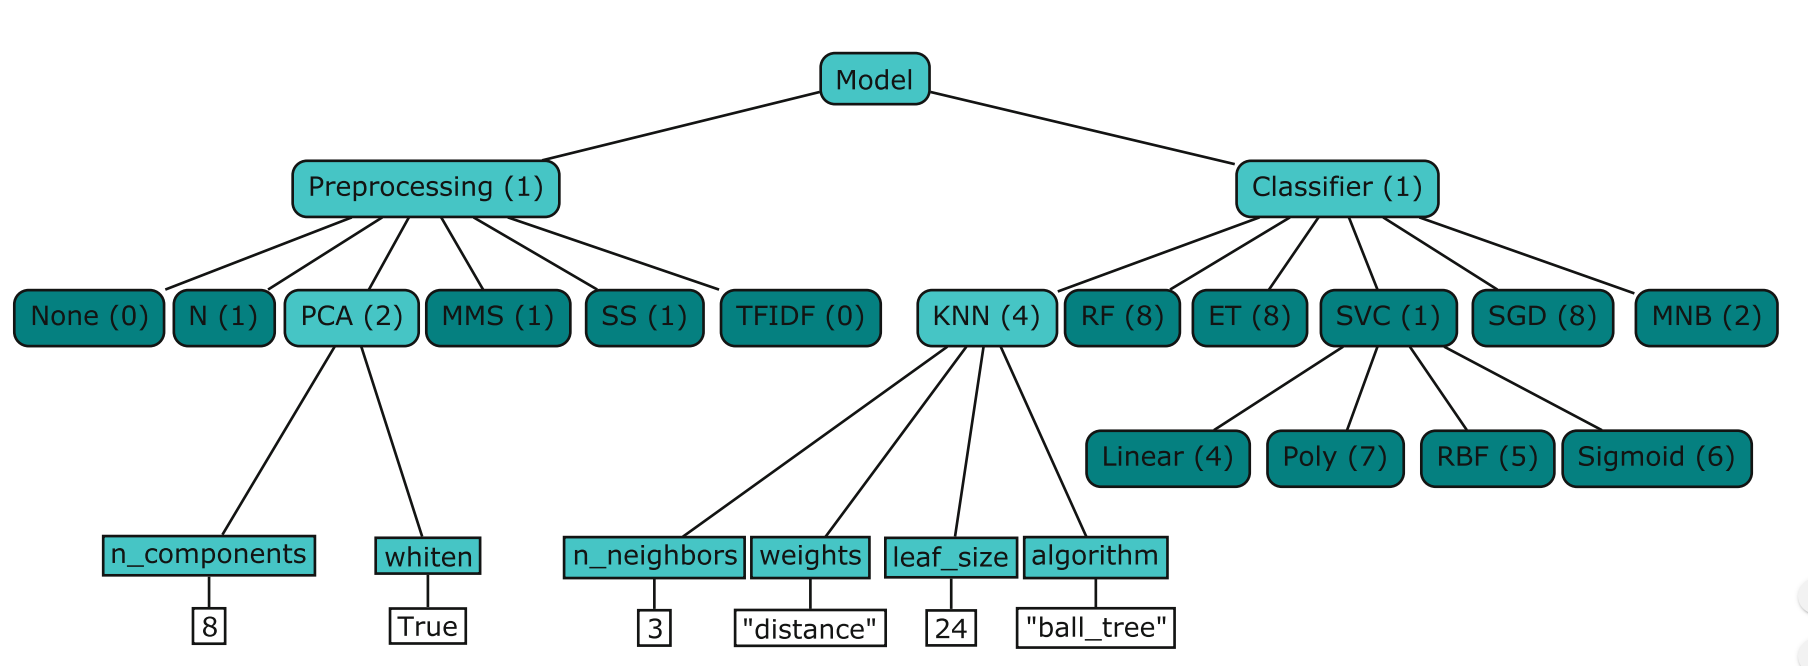
\includegraphics[width=.9\linewidth, height=0.9\textheight, keepaspectratio=true]{images/categ_cond_params/Conditional_Parameters_AutoML_Book.png}
    \newline
    Example of a structured search space (Source: Figure 5.1 of the \lit{\href{https://www.automl.org/wp-content/uploads/2019/05/AutoML_Book.pdf}{AutoML book}})
\end{center}
\end{frame}
%-----------------------------------------------------------------------
\begin{frame}[c]{Structured Search Spaces: Categorical Hyperparameters}

\begin{columns}[T]
\column{0.65\textwidth}

\medskip
Properties of categorical hyperparameters:
\begin{itemize}
    \item \alert{Finite, discrete} set of values
    \item \alert{No natural order} between values 
    \item Potentially different distances between values
\end{itemize}


\column{0.35\textwidth}
\vspace{0.5cm}
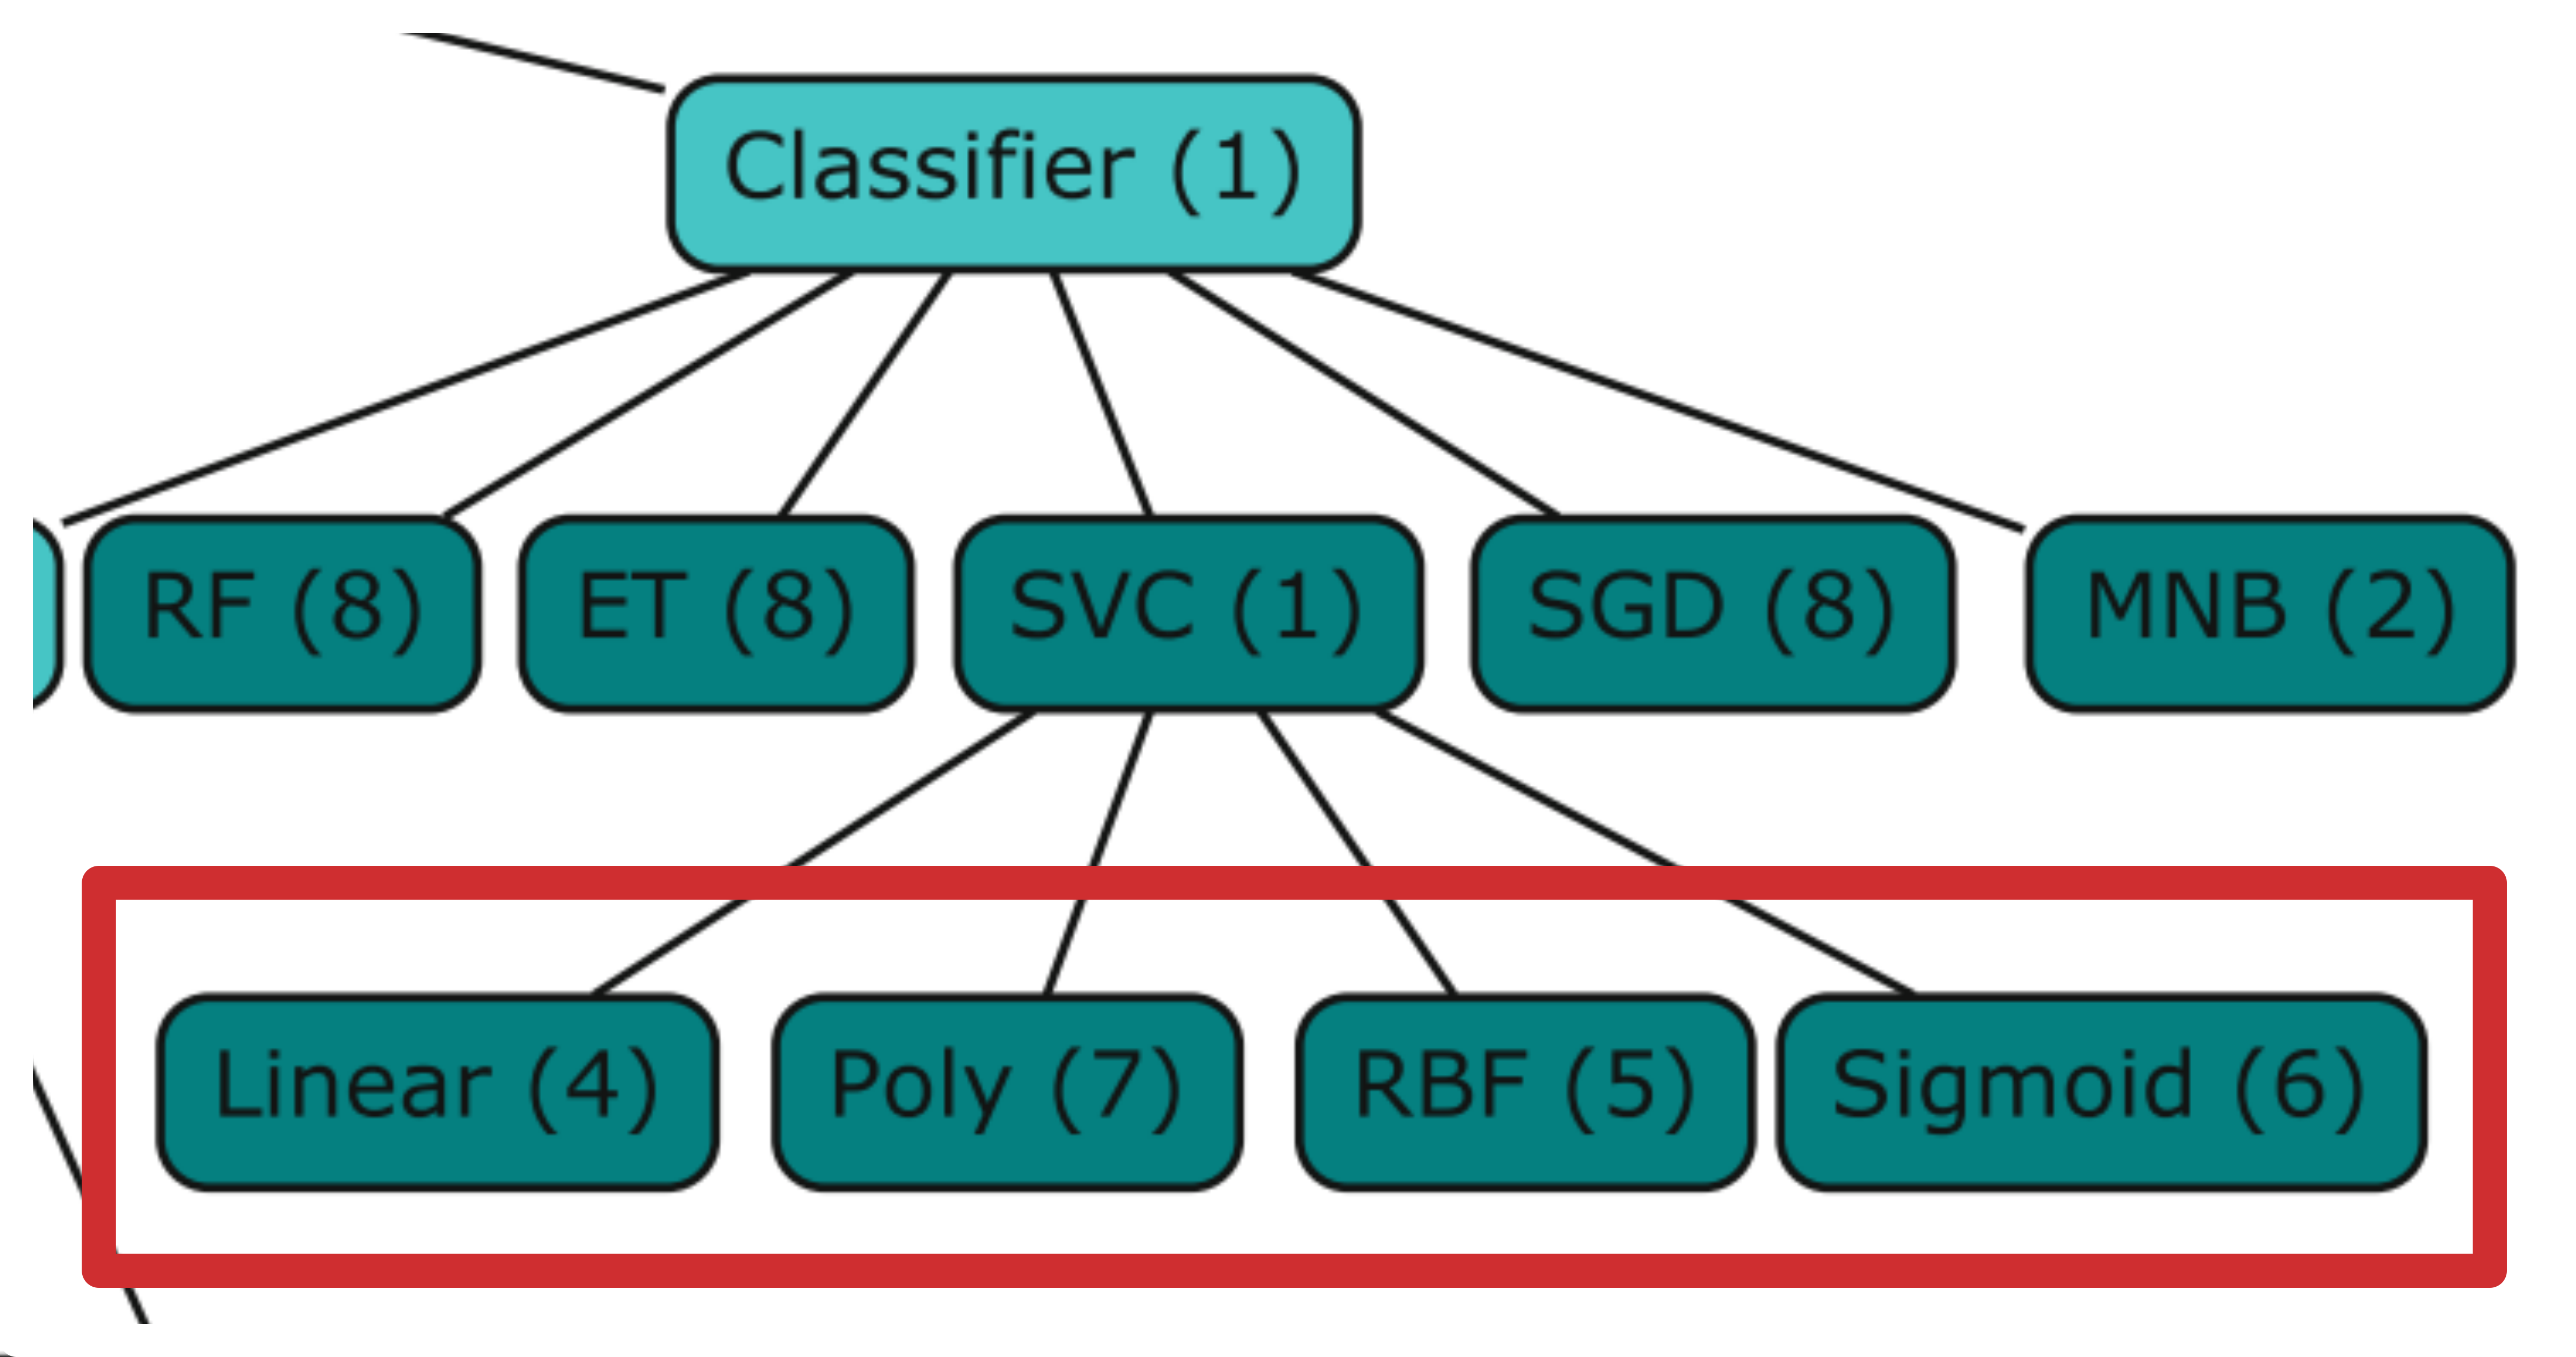
\includegraphics[width=1\textwidth]{images/categ_cond_params/categorical.png}
%
\end{columns}

\pause
\vspace*{-0.4cm}
This has to be taken into account by the surrogate model:
%
\begin{itemize}
    \item Random Forests \alert{natively} handle categorical inputs \lit{\href{https://ml.informatik.uni-freiburg.de/papers/11-LION5-SMAC.pdf}{Hutter et al, 2011}}
    \item \emph{One-hot} encoding provides a simple general solution
    \item Gaussian Processes can use a (weighted) \alert{Hamming Distance Kernel} \lit{\href{https://www.cs.ubc.ca/~hutter/papers/Hutter09PhD.pdf}{Hutter 2009}}:
\vspace*{-0.2cm}
\begin{equation*}
    \kernel_{\theta}(\conf_i, \conf_j) = \exp{\sum_{l=1}^d (-\theta \cdot \delta(\hyperparam_{i,l} \neq \hyperparam_{j,l}))}
\end{equation*}

\vspace*{-0.2cm}
\item Neural networks can learn \alert{entity embeddings} for categorical inputs \lit{\href{https://arxiv.org/pdf/1604.06737.pdf}{Guc et al. 2016}}
\end{itemize}
%
\end{frame}
%-----------------------------------------------------------------------
\begin{frame}[c]{Structured Search Spaces: Conditional Hyperparameters}


\begin{columns}[T]
\column{0.65\textwidth}
\vspace*{0.2cm}
Conditional hyperparameters:
\begin{itemize}
    \item Are \alert{only relevant if} certain other hyperparameters take on certain values
    \item \alert{Should be ignored} by the model \alert{if not active}
\end{itemize}

\column{0.35\textwidth}
\vspace{0.5cm}
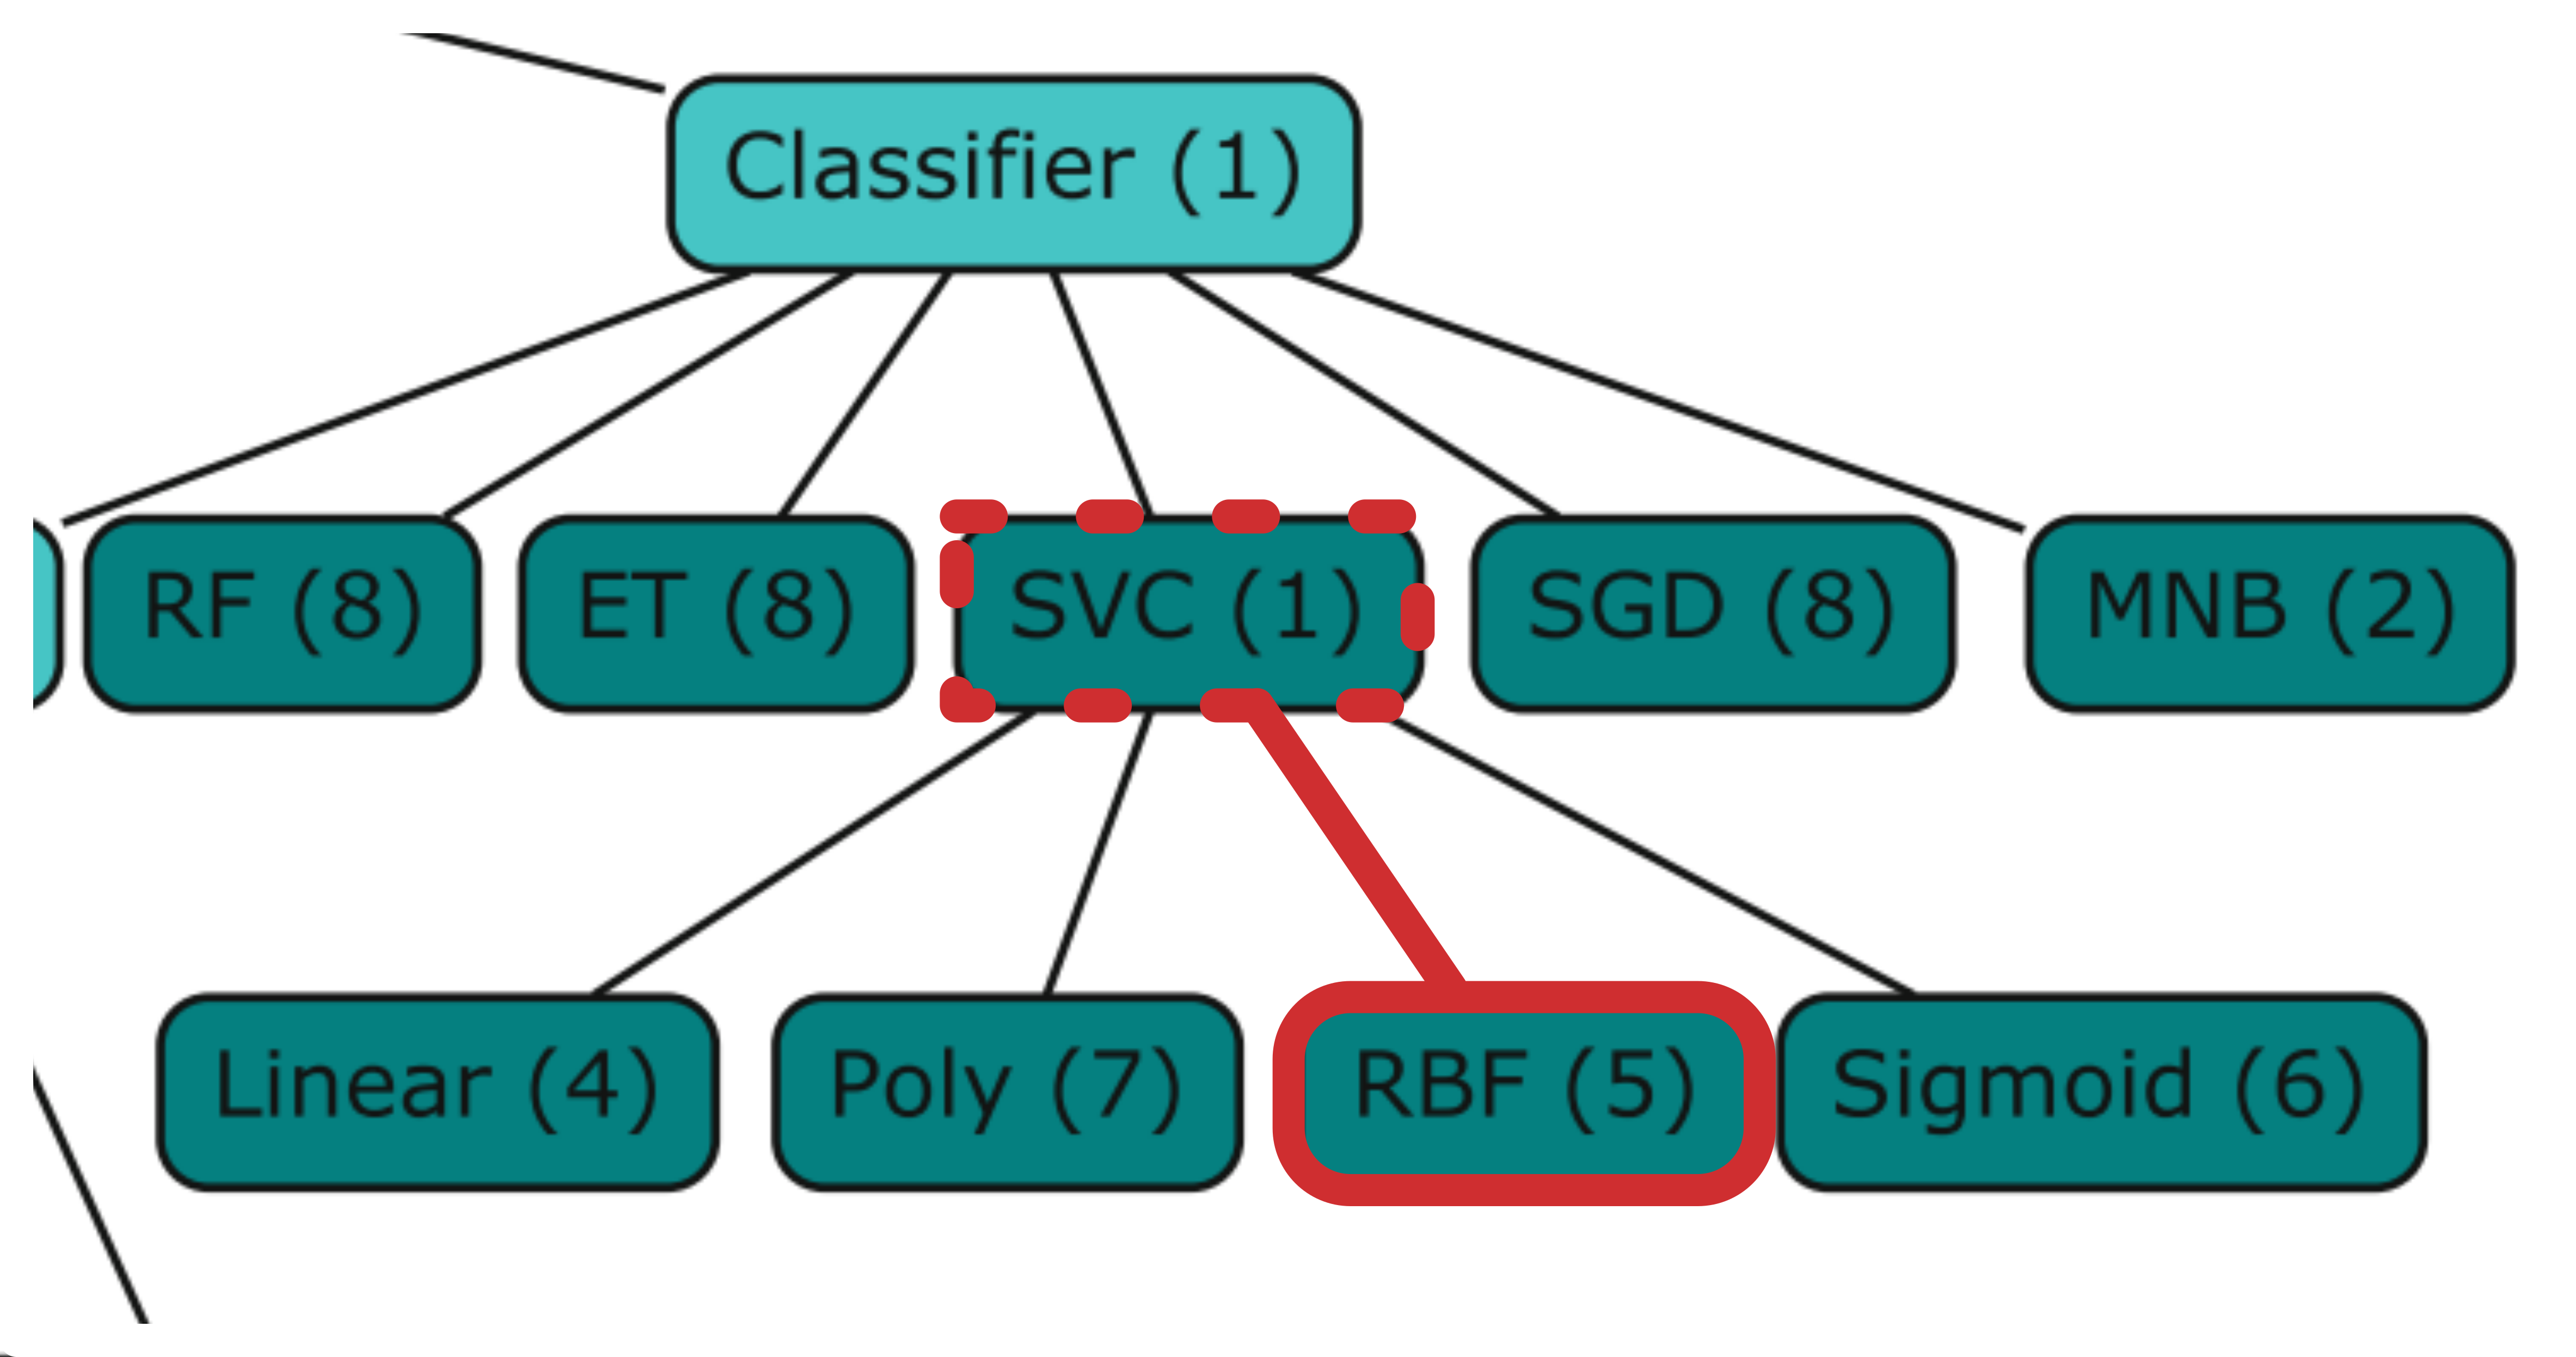
\includegraphics[width=1\textwidth]{images/categ_cond_params/conditional.png}
%
\end{columns}

\pause 
\vspace*{-0.2cm}
Modelling conditional hyperparameters:
\begin{itemize}
    \item Setting the values for inactive hyperparameter to a specific value (e.g. $0$)
    \item Random Forests \lit{\href{https://ml.informatik.uni-freiburg.de/papers/11-LION5-SMAC.pdf}{Hutter et al. 2011}} and Tree Parzen Estimators \lit{\href{http://papers.nips.cc/paper/4443-algorithms-for-hyper}{Bergstra et al. 2011}} can \alert{natively} handle conditional inputs
    \item There exist \alert{several kernels for Gaussian Processes} to handle conditional inputs \lit{\href{https://arxiv.org/abs/1310.5738}{Hutter et al. 2013}} \lit{\href{https://www.etsmtl.ca/Unites-de-recherche/LIVIA/Recherche-et-innovation/Publications/Publications-2017/Levesque_ijcnn_2017.pdf}{Lévesque et al. 2017}} \lit{\href{http://proceedings.mlr.press/v70/jenatton17a.html}{Jenatton et al. 2017}} 
\end{itemize}
%
\pause
\vspace{0.4cm}
Overall, structured search spaces are \alert{still an active research topic} and far from solved
\end{frame}

%-----------------------------------------------------------------------
\begin{frame}[c]{High Dimensions}
\begin{columns}[T]
\column{0.65\linewidth}
	\begin{itemize}
		\item Issues
		\begin{itemize}
			\item Standard Gaussian processes \\ do not tend to fit well in high dimensions
			\item Maximizing the acquisition function \\ is computationally challenging
		\end{itemize}
		\smallskip
		\onslide<2->{
			\item There is still hope
			\begin{itemize}		
				\item Many optimization problems have\\ \alert{low effective dimensionality}
				\item Not all dimensions interact with each other
			\end{itemize}
		}
		\onslide<3->{
			\smallskip
			\pause		
			\item Possible solutions
			\begin{itemize}
			
				\item Optimize in a lower-dimensional \\
				embedding \lit{\href{https://ml.informatik.uni-freiburg.de/papers/16-JAIR-REMBO.pdf}{Wang et al. 2016}}
				\item Fit additive models on subsets \\ of dimensions \lit{\href{http://proceedings.mlr.press/v37/kandasamy15.pdf}{Kandasamy et al. 2015}}
				\item Use other models; e.g., random forests
			\end{itemize}
		}
	\end{itemize}

    \column{0.35\linewidth}

%\bigskip
	{\onslide<2->{
	    \begin{figure}
	    	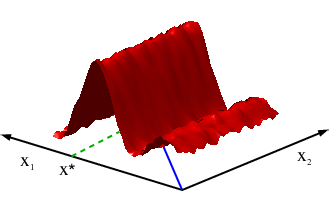
\includegraphics[width=0.8\textwidth]{images/highdim_images/Random_embeddings_in_a_nutshell1.png}\\
	    \end{figure}
    }}
%\bigskip
	{\onslide<3->{
	    \begin{figure}
	    	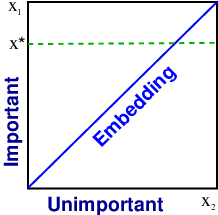
\includegraphics[width=0.65\textwidth]{images/highdim_images/Random_embeddings_in_a_nutshell2.png}
	    \end{figure}
    }}

\end{columns}    
	
\end{frame}
%-----------------------------------------------------------------------



\begin{frame}[c]{Parallel Bayesian Optimization: Multi-point Acquisition Functions}

\begin{itemize}
    \item Often, we have many parallel compute units
    \item How should these be exploited in (the typically inherently sequential) Bayesian optimization?
\medskip
\pause
    \item To select a batch of $q$ points in parallel, we need to compute the multi-point acquisition function.
    E.g., for expected improvement:
    \begin{equation*}
        q\text{-EI}(\conf_{1, \dots, q}) = \E \left[ \cost(\incumbent) - \min_{i=1, \dots, q} \surro(\conf_i) \right]
    \end{equation*}
\pause
\medskip
    \item For EI and KG, this requires \emph{expensive-to-compute} q-dimensional Gaussian cumulative distributions \lit{\href{https://hal.archives-ouvertes.fr/hal-00260579/document}{Ginsbourger et al. 2007}}, \lit{\href{https://arxiv.org/pdf/1606.04414v4.pdf}{Wu et al. 2018}}, \lit{\href{https://arxiv.org/pdf/1602.05149.pdf}{Wang et al. 2019}}
    \pause
    \item Nevertheless, multi-point acquisition functions can be optimized efficiently with gradient descent via the reparameterization trick \lit{\href{https://papers.nips.cc/paper/8194-maximizing-acquisition-functions-for-bayesian-optimization}{Wilson et al. 2018}}
\end{itemize}
\end{frame}


%----------------------------------------------------------------------
\begin{frame}[c]{Asynchronous Parallel Bayesian Optimization with Pending Evaluations}

\begin{itemize}
    \item In practice, typically, not all function evaluations take the same amount of time
    \begin{itemize}
        \item Thus, we need to select \alert{some new points} while we're still waiting for \alert{pending evaluations} at other points
    \end{itemize}
\pause
\bigskip
%
    \item Simple solution: \alert{hallucinate observations for pending evaluations}, and use otherwise standard methods:
    \pause
    \begin{itemize}
        \item \alert{Constant Liar}: Choose a fixed value (constant) \lit{\href{http://www.cs.ubc.ca/labs/beta/EARG/stack/2010_CI_Ginsbourger-ParallelKriging.pdf}{Ginsbourger et al. 2010}}
\smallskip
\item \alert{Kriging Believer}: Use the current mean prediction (belief)  \lit{\href{http://www.cs.ubc.ca/labs/beta/EARG/stack/2010_CI_Ginsbourger-ParallelKriging.pdf}{Ginsbourger et al. 2010}}
\smallskip
\item \alert{Monte Carlo Fantasies} 
        \pause
        \begin{itemize}
            \item Sample pending evaluations from the model
            \item Update copy of the model with these samples
            \item Compute acquisition function under each updated copy 
            \item Define acquisition function as an average over these sampled acquisition functions
%            (fantasies, more details on the next slide).
        \end{itemize}
    \end{itemize}
\end{itemize}

\end{frame}
%----------------------------------------------------------------------
\iffalse
\myframetop{Asynchronous Parallel Bayesian Optimization with Pending Evaluations}{
    %
    Assume we have observed data $\left\{ \left\langle \bonextsample, \bonextobs \right\rangle \right\}^{N}_{\bocount = 1}$ and $J$ evaluations are pending $\left \{\conf_{j} \right \}^{J}_{j = 1}$. We can compute the expected mean function using the following integral: \fhpause
    \begin{equation*}
    \begin{aligned}
        \Bar{\acq} \left( \conf; \left\{ \left\langle \bonextsample, \bonextobs \right\rangle \right\}^{N}_{\bocount = 1}, \left \{\conf_{j} \right \}^{J}_{j = 1} \right) =  \fhpause
        \int_{\mathbb{R}^J}  \acq \left( \conf; \left\{ \left\langle \bonextsample, \bonextobs \right\rangle \right\}^{N}_{\bocount = 1}, \left \{ \left\langle \conf_j, \obs_j \right\rangle \right \}^{J}_{j=1} \right) \\
        p( \{ \obs_j \}^{J}_{j = 1}  \rvert \{ \conf_j \}^{J}_{j = 1}, \left \left\{ \left\langle \bonextsample, \bonextobs \right\rangle \right\}^{N}_{\bocount = 1} )d\obs_1 \dots d\obs_J
    \end{aligned}
    \end{equation*}
    %
    \vspace{-0.8cm}
    \begin{columns}
    \column{0.6\textwidth}
    \only<4->{
    \begin{enumerate}
        \only<4->{\item Evaluated observations: $\left \{\conf_1, \conf_3, \conf_4 \right \}$, pending: $\left \{\conf_2, \conf_5 \right \}$.}
        \only<5->{\item Fit a model for each possible realization of $\left \{\cost(\conf_2), \cost(\conf_5) \right \}$.}
        \only<6->{\item Calculate acquisition function for each model.}
        \only<7->{\item Integrate all acquisition functions over $\conf$.}
    \end{enumerate}
    }
    
    \column{0.4\textwidth}
        \only<4-5>{
        \begin{figure}
            \centering
            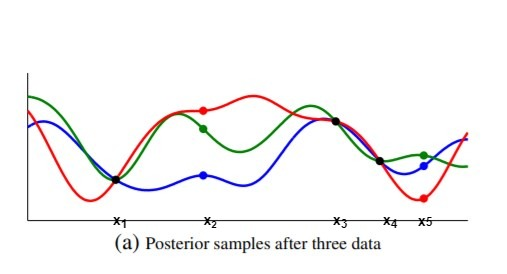
\includegraphics[width=0.8\textwidth]{images/parallel/parallel_a.jpg}
        \end{figure}
        }
        \only<6>{
        \begin{figure}
            \centering
            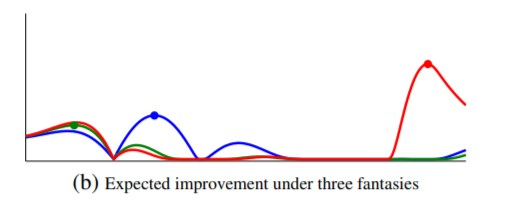
\includegraphics[width=0.8\textwidth]{images/parallel/parallel_b.jpg}
        \end{figure}
        }
        \only<7->{
        \begin{figure}
            \centering
            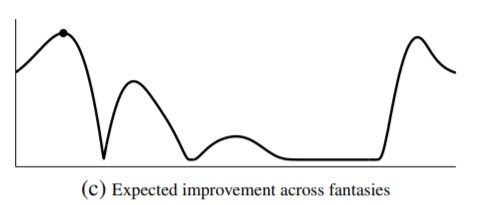
\includegraphics[width=0.8\textwidth]{images/parallel/parallel_c.jpg}
        \end{figure}
        }
    \end{columns}
    
    \source{\href{https://papers.nips.cc/paper/4522-practical-bayesian-optimization-of-machine-learning-algorithms.pdf}{Snoek et al. 2012}}

\vspace*{-0.4cm}
% \notefh{As I mentioned in class, I think the EI plot is wrong; it needs to be zero at the points where fantasies are being evaluated. Can you code this up and make a proper plot this week? Otherwise, I would drop this slide.}

}
\fi
%
%\begin{frame}
%\begin{itemize}
%    \item <+-> Utilize tractable properties of GP to get Monte Carlo estimates of %acquisition function under different results from pending function evaluations. \fhpause
%    \item <+-> Consider the case where $N$ evaluations have completed, with data $\left \{\bonextsample, \bonextobs \right \}^{N}_{\bocount = 1}$ and $J$ evaluations are pending $\left \{\conf_{j} \right \}^{J}_{j = 1}$: \fhpause
%    \begin{equation*}
%        \begin{aligned}
%            \hat{\acq} ( \conf; \left \{ \bonextsample, \bonextobs \right \}, \left \{ \conf_j \right \} ) =  \fhpause
%            \int_{\mathbb{R}^J}  \fhpause \acq ( \conf; \left \{ \bonextsample, %\bonextobs \right \}, \left \{ \conf_j, \obs_j \right \} ) \\  \fhpause
%            p(\left \{ \obs_j \right \}^{J}_{j = 1}  \rvert \left \{ \conf_j \right \}^{J}_{j = 1}, \left \{ \bonextsample, \bonextobs \right \}^{N}_{\bocount=1} )d\obs_1 \dots d\obs_J
%        \end{aligned}
%    \end{equation*}
%\end{itemize}

%\source{\href{https://csc2541-f17.github.io/}{Scalable and Flexible Models of Uncertainty, University of Toronto}}

%\end{frame}
%-----------------------------------------------------------------------
\iffalse
\begin{frame}[c]{Noisy Evaluations}

    \begin{columns}[T]
    
        \column{0.6\textwidth}
    
        \myit{
            \item The probabilistic model natively supports Gaussian noise
            \myit{
                \item A good hyperprior for the noise variance might be needed to robustly determine the right size of the noise
                \item Noise that is not Gaussian (and not Student t \lit{\href{https://www.asc.ohio-state.edu/santner.1/TJS-BJW-WIN/master-driver.pdf}{Santner et al, 2014}}) would require approximations 
            }
        }
    
        \column{0.4\textwidth}
        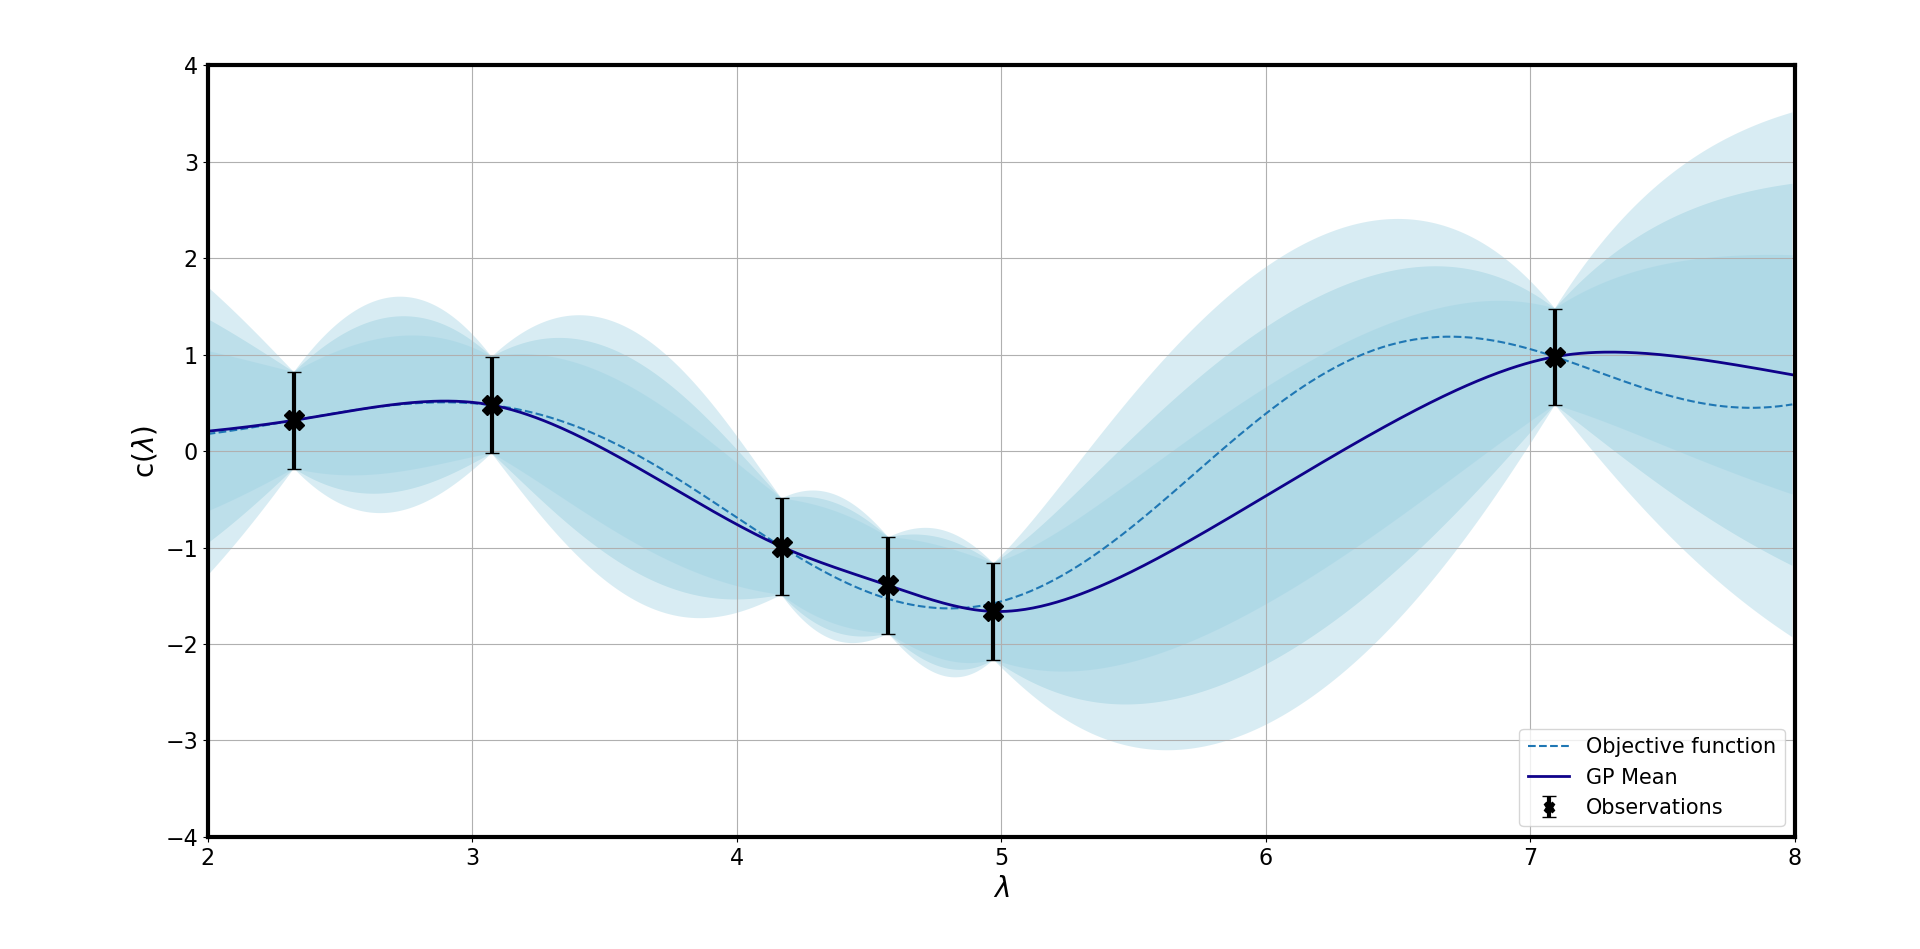
\includegraphics[width=\textwidth]{images/extensions/BO_Loop_Noisy3.png}
        
    \end{columns}
    %        Given noisy evaluations, GP regression proceeds similarly to the noiseless case by adding the variance to the diagonal of the covariance matrix.
    %        \vspace{-0.2cm}
    %        \item KG and ES directly handle noisy function evaluations~\lit{\href{https://arxiv.org/abs/1807.02811}{Frazier 2018}}.
    %        \vspace{-0.2cm}
    
\fhpause
\bigskip
    \myit{
        \item The acquisition function might need adaptation
        \myit{
            \item LBC, TS, ES, and KG, are not affected
            \item PI and EI are based on an the cost $\cost_{inc}$ of the incumbent; it is unclear how to compute this
            \begin{itemize}
                \item Uncertainty about which point is the current incumbent 
                \item Uncertainty about the costs $\cost(\conf_i)$.
                \item \alert{Noisy Expected Improvement}~\lit{\href{https://arxiv.org/abs/1706.07094}{Letham et al. 2019}} extends  regular EI by integrating over the predictive posterior of the model using Monte Carlo
            \end{itemize}
        }
    %        Computing EI with observation noise is challenging:
    %        \vspace{-0.2cm}
}
    

%\begin{itemize}
%    \item Noisy Expected Improvement~\lit{\href{https://arxiv.org/abs/1706.07094}{Letham et al. 2019}} extends the regular Expected Improvement by integrating over the predictive posterior of the model:
%    % There's an additional paper by Gramacy and Lee from 2011 which does a more complicated treatment of noise in EI
%    \begin{equation*}
%        \acq_{NEI}(\conf|\dataset)=\int_{\surro}\acq_{EI}(\conf|\surro)p(\surro|\dataset)\text{d}\surro
%    \end{equation*}
%    \vspace{-0.2cm}
%    \begin{itemize}
%        \item Compute with Monte Carlo Integration.
%        \item Each sample from the model posterior has its own incumbent $\incumbent[\bocount-1]$.
%    \end{itemize}
%    \end{itemize}
\end{frame}
\fi
%----------------------------------------------------------------------

\begin{frame}[c]{Bayesian Optimization with Constraints}

\begin{columns}[T]

\column{0.6\textwidth}

Several types of constraints 
% \notefh{Four? There are 3 listed here. Also, from the description here I don't see a difference between unknown and hidden constraints, just that in the unknown case you're trying to model them!? @Matthias: this might be most efficient to discuss on the phone.}
\begin{small}
\begin{enumerate}
    \item \alert{Known constraints}:\\ can be accounted for when optimizing $\acq$
    %\item Policy constraints: function value is observed, but deemed forbidden~\lit{\href{https://www.soe.ucsc.edu/sites/default/files/technical-reports/UCSC-SOE-10-10.pdf}{Lee and Gramacy 2010}}
    \item \alert{Hidden constraints}: no function value is observed due to a failed function evaluation~\lit{\href{https://www.soe.ucsc.edu/sites/default/files/technical-reports/UCSC-SOE-10-10.pdf}{Lee and Gramacy 2010}}
    \item \alert{Unknown constraints}: there's an additional, but unknown constraint function (e.g., memory used), which can be observed and modeled
\end{enumerate}
\end{small}

\column{0.35\textwidth}
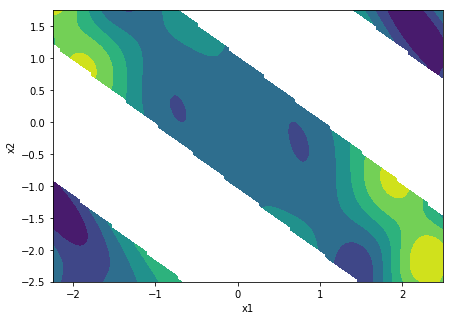
\includegraphics[width=0.9\textwidth]{images/extensions/notebooks_constrained_bo_4_0.png}\\
\vspace*{-0.5cm}
\begin{center}
	%Hidden constraints. 
	\footnotesize{Image source: \lit{\href{https://gpflowopt.readthedocs.io/en/latest/notebooks/constrained_bo.html}{GPFlowOpt Tutorial, Apache 2 License}}}
\end{center}	
\end{columns}

\vspace*{0.2cm}
\pause

Most general solution: \alert{Expected Constrained Improvement}~\lit{\href{https://www.soe.ucsc.edu/sites/default/files/technical-reports/UCSC-SOE-10-10.pdf}{Lee and Gramacy 2010}}:
\vspace{-0.1cm}
\begin{equation}
\nonumber    \alert{ECI(\conf) = EI(\conf)h(\conf)},
\end{equation}
\vspace{-0.1cm}
\noindent{}where $h(\conf)$ is the probability that $\conf$ is a valid configuration.

\vspace{0.4cm}
Further literature in \lit{\href{https://arxiv.org/abs/1807.02811}{Frazier 2018}} and \lit{\href{https://link.springer.com/chapter/10.1007/978-3-030-05318-5_1}{Feurer and Hutter 2019}}.

\end{frame}
%----------------------------------------------------------------------
\begin{frame}[c]{Even more extensions}
Bayesian optimization has been extended to numerous scenarios:
\begin{itemize}
    \item Multi-task, Multi-fidelity and Meta-learning $\rightarrow$ separate lecture
    \item Multi-objective Bayesian optimization $\rightarrow$ separate lecture
    \item Bayesian optimization with safety guarantees~\lit{\href{http://proceedings.mlr.press/v37/sui15.pdf}{Sui et al. 2015}}
    \item Directly optimizing for ensemble performance~\lit{\href{http://auai.org/uai2016/proceedings/papers/73.pdf}{Lévesque et al. 2016}}
    \item Combination with local search methods~\lit{\href{https://www.researchgate.net/publication/241216681_Bayesian_Guided_Pattern_Search_for_Robust_Local_Optimization}{Taddy et al. 2009}}~\lit{\href{https://papers.nips.cc/paper/8788-scalable-global-optimization-via-local-bayesian-optimization.pdf}{Eriksson et al. 2019}}
    \item Optimization of arbitrary spaces that can be described by a kernel (e.g., neural network architectures~\lit{\href{https://papers.nips.cc/paper/7472-neural-architecture-search-with-bayesian-optimisation-and-optimal-transport.pdf}{Kandasamy et al. 2018}} or 
    %a latent embedding, such as
    molecules~\lit{\href{https://arxiv.org/abs/1709.05501}{Griffiths et al. 2017}})
    \item Many more (too many to mention)
\end{itemize}
  
\end{frame}
%-----------------------------------------------------------------------
\begin{frame}[c]{Questions to Answer for Yourself / Discuss with Friends}

\begin{itemize}
% Categorical and Conditional
\item \alert{Discussion.} What would happen if you treat a categorical hyperparameter as continuous (e.g., $\{A, B, C\}$ as $\{0, 0.5, 1\}$), in Bayesian optimization using a Gaussian Process?
\medskip
% Parallel
\item \alert{Repetition.} Which methods can you use to impute values for outstanding evaluations? What are advantages and disadvantages of each method?
\medskip
% Noise & Constrained
\item \alert{Discussion.} What are worst case scenarios that could happen if you ignore the noise during Bayesian optimization?
% Further
\end{itemize}
\end{frame}
\end{document}